%%%%%%%%%%%%%%%%%%%%%%%%%%%%%%%%%%%%%%%%%%%
\newpage
\chapter{Discrete Dislocation Dynamics  in MoDELib}



\section{Topology of dislocation networks}

\subsection{Topological operations}



The objective of this chapter is to give an overview of the DDD method, and to describe its implementation in the MoDELib library. 

DDD is a simulation method to study the plastic deformation of crystalline materials due to the motion of dislocations. 
It is a hybrid discrete-continuum simulation method, which  in the multiscale modeling framework bridges   atomistic  methods (e.g. Molecular Dynamics) and continuum methods (e.g. Finite Element Crystal Plasticity). 
Its hybrid character is due to the fact that crystal dislocations are represented discretely (individually), although their interactions are computed semi-analytically using continuum elasticity and without atomistic degrees of freedom.
 
DDD simulation typically take place in a spatial domain representing either a finite or a periodic material volume. Fig.~\ref{DDDnutshellA} shows a snapshot of a typical MoDELib DDD simulation, where individual dislocation lines are colored according to their Burgers vector, and the intensity of the shaded background represents the local slip due to their motion.  A minimal DDD algorithm is reported in Fig.~\ref{DDDnutshellB}. 


\SetKwFor{MyFor}{main loop}{}{end}
\SetKwFor{MyInit}{initialization:}{}{end}
\SetKwFor{MyDisc}{initialize:}{}{end}

\SetKwFor{ForRegion}{\textcolor{blue}{for each region}}{}{end}
\SetKwFor{ForRegionBnd}{\textcolor{blue}{for each region boundary}}{}{end}

 \begin{figure}[h]
 \centering
  \begin{subfigure}{.48\textwidth}
 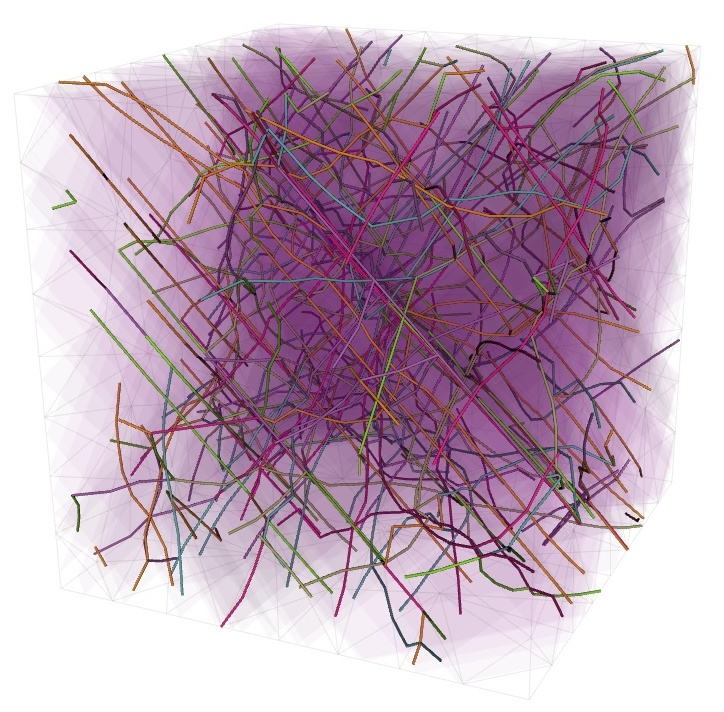
\includegraphics[width=\textwidth]{image_650}
 \caption{sample configuration}
  \label{DDDnutshellA}
\end{subfigure}
  \begin{subfigure}{.48\textwidth}
%\begin{minipage}[t]{0.45\textwidth}
\begin{algorithm}[H]
%\SetAlgoLined
\MyInit{}
 {
simulation domain\;
material properties and slip systems\;
initial dislocation configuration\;
 }
\MyFor{}{
compute mutual dislocation stress\;
add other stress sources\;
compute line velocities from local stress\;
compute  nodal velocities\;
update nodal positions\;
perform discrete events:\\
- junctions\\
- cross-slip\\
- network remeshing\\
- nucleation\\
 }
\end{algorithm}
 \caption{minimal DDD algorithm}
     \label{DDDnutshellB}
\end{subfigure}
  \caption{typical  DDD simulation in MoDELib. }
    \label{DDDnutshell}
 \end{figure}
 
 During the initialization phase a mesh of the simulation domain is prepared, material properties are selected, and an initial dislocation microstructure is generated. In. MoDELib, these processes are automated as explained in section \ref{runningMoDELib}. During the main simulation loop the mutual interaction forces between dislocations are computed using semi-analytical expressions derived from the elastic theory of dislocations described in section \ref{elasticTheoryDislocations}. This is typically the most time-consuming part of a single simulation step. External loads and possibly other stress sources are then added to determine the total force on each line element of a dislocation. Overdamped dynamics is then invoked to compute the local dislocation velocity given the local force, using special functions called \textit{mobility laws}. A Finite Element (FE) scheme is then employed to find the velocity of the discretization points (nodes) which determine the dislocation configuration. Once ta new configuration is obtained through a simple time-marching scheme, a series of processes takes place to update the dislocation topology due to discrete physical events such as collisions, cross slip, etc.

In the remainder of this chapter we develop the necessary theoretical background necessary to understand the  DDD method. We then proceed to the description of the MoDELib implementation. 
